\documentclass{beamer}[fontset=windows]
\usepackage{ctex, hyperref}
\usepackage[T1]{fontenc}
\usepackage[backend=bibtex,bibstyle=gb7714-2015,citestyle=gb7714-2015]{biblatex}
\setlength{\bibitemsep}{3bp}
\addbibresource{ref.bib}
\renewcommand*{\bibfont}{\zihao{5}\linespread{1.27}\selectfont}
\usefonttheme[onlymath]{serif}
% other packages
\usepackage{latexsym,amsmath,xcolor,multicol,booktabs,calligra}
\usepackage{graphicx,pstricks,listings,stackengine}

\author{吴熙楠}
\title{单电子晶体管}
\subtitle{Single Electron Transistor}
\institute{北京大学物理学院}
\date{\today}
\usepackage{PKU}
% defs
\def\cmd#1{\texttt{\color{red}\footnotesize $\backslash$#1}}
\def\env#1{\texttt{\color{blue}\footnotesize #1}}
\definecolor{deepblue}{rgb}{0,0,0.5}
\definecolor{deepred}{rgb}{0.6,0,0}
\definecolor{deepgreen}{rgb}{0,0.5,0}
\definecolor{halfgray}{gray}{0.55}

\lstset{
	basicstyle=\ttfamily\small,
	keywordstyle=\bfseries\color{deepblue},
	emphstyle=\ttfamily\color{deepred},    % Custom highlighting style
	stringstyle=\color{deepgreen},
	numbers=left,
	numberstyle=\small\color{halfgray},
	rulesepcolor=\color{red!20!green!20!blue!20},
	frame=shadowbox,
}


\begin{document}
	
	\kaishu
	\begin{frame}
		\titlepage
    \begin{figure}[htpb]
    	\begin{center}
    		
\includegraphics[width=0.2\linewidth]{pic/PKU_logo.png}
    	\end{center}
    \end{figure}
	\end{frame}
	
	\begin{frame}
		\tableofcontents[sectionstyle=show,subsectionstyle=show/shaded/hide,subsubsectionstyle=show/shaded/hide]
	\end{frame}
	\section{单电子晶体管的基本概念}
    \begin{frame}
    \begin{block}{量子隧穿}
    	\begin{figure}[H]
    		\centering
    		\hspace{2em}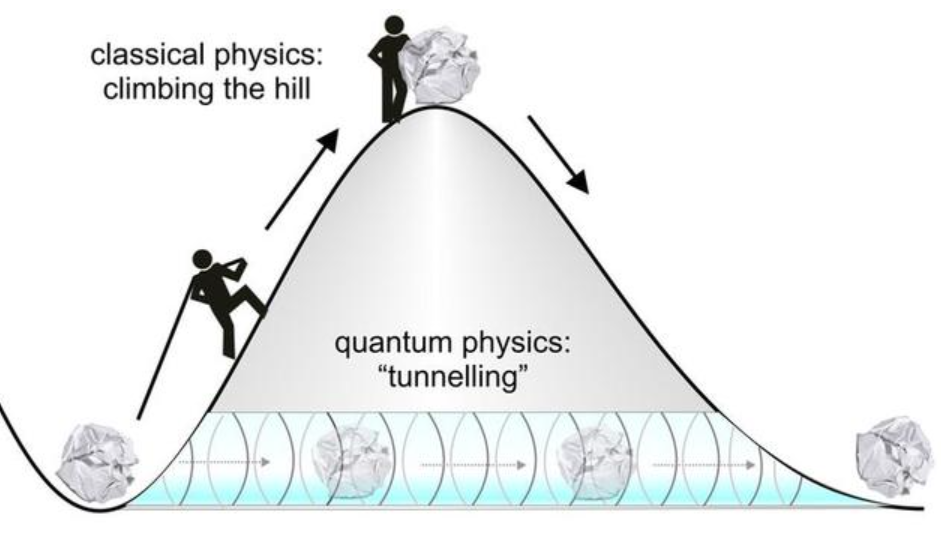
\includegraphics[width=.6\linewidth]{pic/1.png}
    		\caption{量子隧穿效应图示
    		}
    	\end{figure}
        \begin{itemize}
        \item 当两个金属电极被厚度仅为$\sim 1nm$的绝缘势垒隔开时,费米能量下的电子即使能量太低而无法克服绝缘区的大势垒,也能通过绝缘体,形成经典运动。
        \end{itemize}
    \end{block}
    \end{frame}
    \begin{frame}
        \begin{block}{SET的一般结构}
            	\begin{figure}[H]
            		\centering
            		\hspace{2em}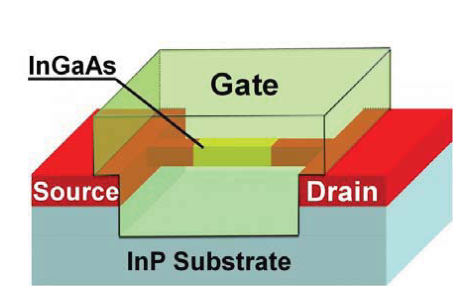
\includegraphics[width=.5\linewidth]{pic/3.png}
            		\caption{SET的一般结构\cite{mandal2013single}
            		}
            	\end{figure}
        \begin{itemize}
                 \item\small{ 在这个$SET$中通过绝缘体与金属电极分开(在这个例子中是$InP$)。$InP$中掺杂了$Si$,从而提供电子。它们落入$InGaAs$,因为它们的能量在后者中更低。硅原子上产生的正电荷产生了一个势,将电子保持在$InGaAs/InP$界面上,形成二维电子气体。}
                 \end{itemize}
        \end{block}
        \end{frame}
    \begin{frame}
    \begin{block}{SET的等效电路}
        	\begin{figure}[H]
        		\centering
        		\hspace{2em}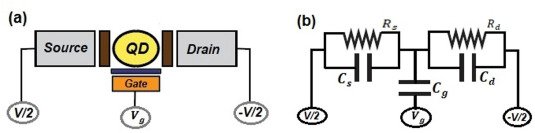
\includegraphics[width=1.0\linewidth]{pic/2.jpg}
        		\caption{(a)SET的结构示意图;(b)SET的等效电路\cite{MOULHIM2020114078}
        		}
        	\end{figure}
    \end{block}
    \end{frame}
    \begin{frame}
    \begin{block}{单电子晶体管与传统晶体管}
    \begin{itemize}
    \item 传统的场效应晶体管是一种开关,当电子添加到半导体时,它会打开,当电子移除时,它会关闭。这些开和关状态给出数字计算机计算所需的1和0,这些晶体管在物理学上几乎完全是经典的,只有少数几个表征它们行为的数字受到量子力学的影响。然而,我们将电子限制在一个小体积内,并通过隧道与导线通信,每次添加一个电子时,它就会再次打开和关闭,我们称之为单电子晶体管($SET$),该装置的行为完全是量子力学的。
    \item 开关装置:使用受控电子隧穿来放大电流;晶体管:一次传导一个电子的电流。
    \item 单电子晶体管相比传统晶体管能做到更薄,而且也更低功耗。
    \end{itemize}
    \end{block}
    \end{frame}
    \section{单电子晶体管的基本原理}
    \begin{frame}
    \begin{block}{球形量子点($QD$)}
    \begin{itemize}
    \item $E=\dfrac{\pi^{2}\hbar^{2}}{2ma^{2}}(n_{x}^{2}+n_{y}^{2}+n_{z}^{2})=\dfrac{\hbar^{2}\chi_{n,l}^{2}}{2m}(\dfrac{4\pi}{3})^{2/3}V^{-2/3}$
    \item $E_{e-e}=\dfrac{1}{2}\dfrac{N(N-1)e^{2}}{4\pi \epsilon a}\quad(C_{\sum}=4\pi\epsilon a)$
    \item 球形量子点中的总能量:$U_{N}=\sum\limits_{i=1}^{N}E_{i}+E_{e-e}$
    \item 定义$\mu(N)$为量子点电子数由$N-1$增加到$N$时需要的能量,则:$\mu(N)=E_{N}+(N-1)\dfrac{e^{2}}{C_{\sum}}$
    \item $\mu(N+1)=\mu(N)+\Delta E+E_{c}(\Delta E=E_{N+1}-E_{N},E_{c}=\dfrac{e^{2}}{C_{\sum}})$
    \item $\Delta \mu=\Delta E+E_{c}$
    \end{itemize}
    \end{block}
    \end{frame}
    \begin{frame}
    \begin{block}{$SET$工作的条件}
    \begin{itemize}\small{
    \item 在给定的温度下,晶体中声子的能量或热能可以用$k_{B}T$来计算。在$SET$中,热能可以用来激发电子到更高的能量,从而使电子有能力隧穿结势垒。只有当热能大于充电能量的总和时才会发生,因此$SET$在给定温度下工作的第一个条件是:$E_{add}=\Delta E+E_{c}>>k_{B}T$
    \begin{itemize}
    \item 经典库伦封锁:$\Delta E<<k_{B}T<<E_{c}$;量子库伦封锁:$k_{B}T<<\Delta E,E_{c}$
    \end{itemize}
    \item 我们需要考虑隧穿电阻受电子给量子点充电的时间的影响,这个时间为$\Delta t=R_{t}C_{\sum}$,称为量子点电容时间常数。而考虑电子作为量子粒子,特定时间范围$\Delta t$下电子能量的不确定度可由测不准原理$E_{e}\approx\dfrac{\hbar}{\Delta t}$计算得到。因此电子能必须小于附加能量,以保证只有隧穿输运现象。最后一个条件为:$R_{t}<<\dfrac{\hbar}{E_{add}C_{\sum}}$
    \begin{itemize}
    \item 在经典库伦封锁下,$\Delta E\sim 0,R_{t}<<\dfrac{\hbar}{e^{2}}\sim 25.8k\Omega$
    \end{itemize}}
    \end{itemize}
    \end{block}
    \end{frame}
    \begin{frame}
        \begin{block}{SET的等效电路}
            	\begin{figure}[H]
            		\centering
            		\hspace{2em}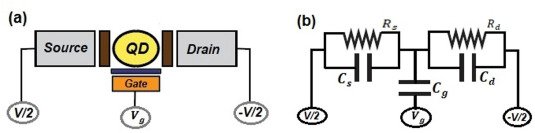
\includegraphics[width=.8\linewidth]{pic/2.jpg}
            		\caption{(a)SET的结构示意图;(b)SET的等效电路\cite{MOULHIM2020114078}
            		}
            	\end{figure}
        \begin{itemize}
        \item\small{ $SET$包含两个隧道结,第一个是通过形成隧道障的隔离材料将源和量子点连接起来,该结的容量为$C_{s}$,隧穿势垒电阻为$R_{s}$。量子点与漏极连接形成的第二个隧穿结的容量为$C_{d}$,隧穿势垒电阻为$R_{d}$,量子点栅的容量为$C_{g}$,其中满足$C_{\sum}=C_{s}+C_{d}+C_{g}$。在源极和漏极之间施加电压时,电子通过隧道势垒穿过量子点从源极到漏极。在栅极上施加电压时,量子点中的电子数发生变化。$SET$的等效电路如上图所示。}
        \end{itemize}
        \end{block}
        \end{frame}
        \begin{frame}
        \begin{block}{电路方程组}
        \begin{itemize}
        \item $-Ne=Q_{s}+Q_{d}+Q_{g}$
        \item $-\dfrac{V}{2}+\dfrac{Q_{s}}{C_{s}}+\dfrac{Q_{g}}{C_{g}}-V_{g}=0$
        \item $-\dfrac{V}{2}+\dfrac{Q_{d}}{C_{d}}-\dfrac{Q_{g}}{C_{g}}+V_{g}=0$
        \end{itemize}
        \end{block}
        \begin{block}{方程组求解}
        \begin{itemize}
        \item $Q_{g}=\dfrac{C_{g}}{C_{\sum}}(\dfrac{V}{2}(C_{s}-C_{d})+V_{g}(C_{s}+C_{d})-Ne)$
        \item $Q_{s}=\dfrac{C_{s}}{C_{\sum}}(V_{g}C_{g}+\dfrac{V}{2}(2C_{d}+C_{g})+Ne)$
        \item $Q_{d}=\dfrac{C_{d}}{C_{\sum}}(-V_{g}C_{g}+\dfrac{V}{2}(2C_{s}+C_{g})-Ne)$
        \end{itemize}
        \end{block}
        \end{frame}
        \begin{frame}
        \begin{block}{对结果的讨论}
        \begin{itemize}
        \item 从源极向量子点增加一个电子$\mu^{+}_{1}(N+1)=\Delta E+\mu(N)+\dfrac{e^{2}}{C_{\sum}}-e\dfrac{V}{2}+e\dfrac{V(C_{s}-C_{d})-2V_{g}C_{g}}{2C_{\sum}}$
        \begin{itemize}
        \item 同理从源极让量子点减少一个电子 $\mu^{-}_{1}(N)=-\mu(N)+e\dfrac{V}{2}+e\dfrac{V(C_{d}-C_{s})-2V_{g}C_{g}}{2C_{\sum}}$
        \end{itemize}
        \item 从漏极向量子点增加一个电子$\mu^{+}_{2}(N+1)=\Delta E+\mu(N)+\dfrac{e^{2}}{C_{\sum}}+e\dfrac{V}{2}+e\dfrac{V(C_{s}-C_{d})-2V_{g}C_{g}}{2C_{\sum}}$
                \begin{itemize}
                \item 同理从漏极让量子点减少一个电子 $\mu^{-}_{2}(N)=-\mu(N)-e\dfrac{V}{2}+e\dfrac{V(C_{d}-C_{s})-2V_{g}C_{g}}{2C_{\sum}}$
                \end{itemize}
        \end{itemize}
        \end{block}
        \end{frame}
    \begin{frame}
    \begin{block}{进一步讨论}
    \begin{itemize}
    \item 我们认为要保持孤电子岛效应,则:$\mu^{+}_{1,2}(N+1),\mu^{-}_{1,2}(N)>0$
    \small{\item $\dfrac{2}{e}[1+\dfrac{C_{d}-C_{s}}{C_{\sum}}]^{-1}[\Delta E+\mu(N)+\dfrac{e^{2}}{C_{\sum}}-e\dfrac{V_{g}C_{g}}{C_{\sum}}]>V>\dfrac{2}{e}[1+\dfrac{C_{d}-C_{s}}{C_{\sum}}]^{-1}[\mu(N)-e\dfrac{V_{g}C_{g}}{C_{\sum}}]$
    \item $\dfrac{2}{e}[\dfrac{C_{d}-C_{s}}{C_{\sum}}-1]^{-1}[\Delta E+\mu(N)+\dfrac{e^{2}}{C_{\sum}}-e\dfrac{V_{g}C_{g}}{C_{\sum}}]>V>\dfrac{2}{e}[\dfrac{C_{d}-C_{s}}{C_{\sum}}-1]^{-1}[\mu(N)-e\dfrac{V_{g}C_{g}}{C_{\sum}}]$}
    \item 这四个不等式方程定义了栅极电压与源漏极电压图中量子库仑封锁的有效区域,从而可以得到施加电压的极限。
    \end{itemize}
    \end{block}
    \end{frame}
    \begin{frame}
    \begin{block}{量子库伦封锁区}
    \begin{figure}[H]
    \centering
    \hspace{2em}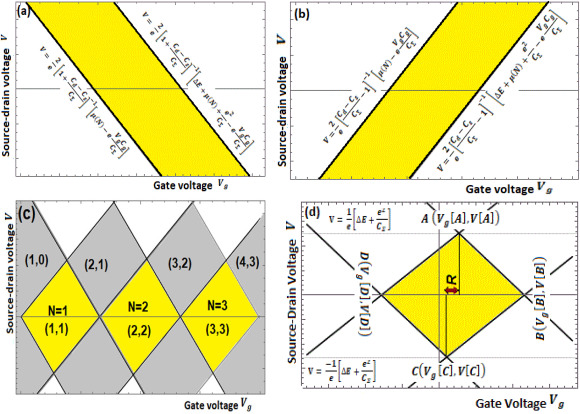
\includegraphics[width=.7\linewidth]{pic/3.jpg}
    \caption{量子库仑封锁区:(a),(b)对上述不等式区域示意图;(c),(d)对于不同的N值所占区域示意图\cite{MOULHIM2020114078}}
    \end{figure}
    \end{block}
    \end{frame}
    \begin{frame}
    \begin{block}{量子库伦封锁区}
    \begin{figure}[H]
    \centering
    \hspace{2em}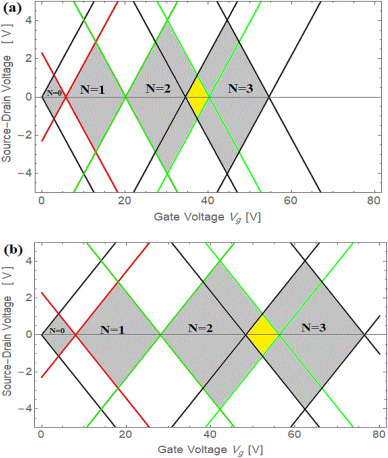
\includegraphics[width=.45\linewidth]{pic/4.jpg}
    \caption{量子库仑封锁区:(a),(b)在不同参数下的量子库伦封锁区\cite{MOULHIM2020114078}}
    \end{figure}
    \end{block}
    \end{frame}
    \begin{frame}
    \begin{figure}[H]
        \centering
        \hspace{2em}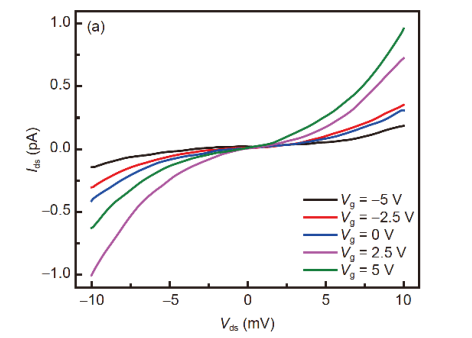
\includegraphics[width=.8\linewidth]{pic/5.png}
        \caption{低温下库伦封锁效应对$I-V$曲线的影响\cite{ali2020single}}
        \end{figure}
    \end{frame}
    \begin{frame}
        \begin{figure}[H]
            \centering
            \hspace{2em}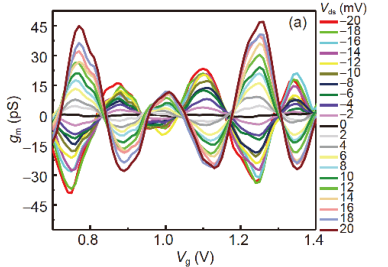
\includegraphics[width=.8\linewidth]{pic/6.png}
            \caption{单电子隧穿效应门限电压影响\cite{ali2020single}}
            \end{figure}
        \end{frame}
    \begin{frame}
    \begin{block}{小总结}
    \begin{itemize}\small{
    \item 由于限制能量依赖于量子点的大小,电子通过量子点隧穿输运的条件反过来取决于量子点的大小。随着量子点半径的减小,量子点的约束能增大,从而使给量子点充电所需的附加电荷能增大,导致热能通过隧道结激发的能力降低。因此,与较大的量子点相比,较小尺寸的量子点为$SET$在高温条件下工作提供了更大的稳定性。
    \item $SET$工作的第二个条件由隧道障壁的高度决定。较小的能量势垒提供较低的隧穿阻力,从而保证电子的隧穿输运过程能够发生。限制能量的增加增加了栅极电压的周期,这意味着$SET$操作获得了较大范围的栅极电压。
    \item 为了获得最大的电导间隙,可以选择合适的栅极电压值。库仑封锁面积随着限制能量的增加而增加,这导致源极电压值范围的增加,阻止电子隧穿。这反过来又增加了电导间隙的宽度,这意味着小尺寸的量子点可以获得宽的电导间隙,这个宽度除了取决于闸极电压外,还取决于$\Delta E$。}
    \end{itemize}
    \end{block}
    \end{frame}
    \section{单电子晶体管中的近藤效应}
    \begin{frame}
    \begin{block}{$Kondo \quad Effect$}
    \begin{itemize}
    \item $\rho=\rho_{i}+\rho(T)$
    \begin{itemize}
    \item $T<<\Theta,\rho\sim T^{5};T>>\Theta,\rho\sim T$
    \end{itemize}
    \item 实验上发现某些掺有磁性杂质原子的非磁性金属的$\rho-T$曲线在低温下出现一个极小值。
    \begin{itemize}
    \item 金属出现电阻极小时,都可测得局域的杂质磁矩,表明电阻反常可能源于杂质磁矩。
    \item 杂质浓度很低($<10^{-6}$)时,电阻仍有反常现象,表明此现象由导电电子和磁性杂质间相互作用所致,与磁性杂质之间的相互作用无关。
    \end{itemize}
    \item 电阻极小值的出现是磁性杂质离子与传导电子气交换耦合作用的结果,交换耦合作用引起传导电子被局域磁性原子散射,使磁性原子自旋反向,传导电子本身也反向;随后,倒向的磁性原子又作用于该传导电子,这一多次散射过程相当于对电子运动的障碍,是使电阻增加的原因。
    \end{itemize}
    \end{block}
    \end{frame}
    \begin{frame}
    \begin{block}{$Kondo\quad Effect\quad in \quad SET$}
    \begin{itemize}
    \item 近藤效应只出现在缺陷是磁性的情况下,换句话说,当杂质原子中所有电子的总自旋是非零时,而SET中的电子数可控,局域态与费米能级之间的距离可以调节。
    \item 如果量子点上的电子数是奇数,那么在低温下,由于近藤效应,两个隧穿结之间的电导会增加。
    \item 我们假设加入一个电子需要的能量为$\epsilon_{0}$,则作为一种量子粒子,自旋向上的电子可以从杂质的位置隧穿出去,在杂质之外短暂地占据一个经典禁止的“虚态”,然后被来自金属的电子所取代,这可以有效地“翻转”杂质的自旋。
    \item 由于不确定关系,持续时间$\Delta t\sim \dfrac{\hbar}{\epsilon_{0}}$,在这个时间尺度内,另一个电子必须通过隧道从费米面返回到杂质,这个电子的自旋可能指向相反的方向。也就是说,杂质的初始态和最终态可以有不同的自旋。
    \end{itemize}
    \end{block}
    \end{frame}
    \begin{frame}
    \begin{block}{$Kondo\quad Effect$发生的前提}
    \begin{itemize}
    \item 量子点系统的参数需满足:\\$\epsilon_{0}<\mu<\epsilon_{0}+U,|\epsilon_{0}-\mu|>>\Gamma,|\epsilon_{0}+U-\mu|>>\Gamma$
    \begin{itemize}
    \item 其中$\Gamma$是电子在量子点和金属电极之间的隧穿率.
    \end{itemize}
    \item 系统所处环境温度须低于$Kondo$温度($T_{k}$),\\$T_{k}=\dfrac{1}{2}(\Gamma U)^{1/2}exp(\pi\epsilon_{0}(\epsilon_{0}+U)/\Gamma U)$
    \item 量子点内电子数N为奇数时,即含局域磁;传导电子能量$E>k_{B}T_{k}$(可观察条件)
    \end{itemize}
    \end{block}
    \end{frame}
    \begin{frame}
    \begin{block}{量子点中发生近藤效应的物理本质}
    \begin{itemize}
    \item 周围自由电子对量子点自旋的屏蔽;
    \item $T<T_{k}$,量子点内未配对的电子与$S/D$电极中的导带态杂化,量子点和电子屏蔽云结合形成准量子点;
    \item 自旋单态:连续自旋反转过程有效地屏蔽了量子点的自旋,形成自旋单态。
    \end{itemize}
    \end{block}
    \begin{block}{近藤共振}
    \begin{itemize}
    \item 量子点内的$Kondo$效应会使电极中的电子态密度在费米能级处出现尖峰, 即近藤共振峰,从而增加电导。
(由于传输特性,如电导是由能量接近费米能级的电子决定的,额外的共振可以极大地改变电导)
    \end{itemize}
    \end{block}
    \end{frame}
    \begin{frame}
    \begin{block}{$Why$}
    \begin{itemize}
    \item 近藤效应能使得源漏极与电子岛更好的混合起来(?);
    \item 非常高的近藤温度$T_{k}> 10 K$(与金属或稀磁性合金的$100 mK\sim1 K$相比);
    \item $SET$是高度可控(通过偏置,磁场等)的器件。
    \end{itemize}
    \end{block}
    \end{frame}
    \section{单电子晶体管的应用}
    \begin{frame}
    \begin{block}{SET的发展历程}
    \begin{itemize}
    \item 1968年就在含有金属粒子的隧道结中首次观察到电荷量子化效应。后来,许多作者提出了可以用栅极电极克服库仑封锁的想法,Kulik 和 Shekhter发展了库仑封锁振荡理论,电导作为栅极电压函数的周期性变化。他们的理论是经典的,包括电荷量子化,但不包括能量量子化。
    \item 1987年,Fulton 和 Dolan 才完全用金属制造了第一个SET,并观察到了预测的振荡。他们制造了一个金属粒子,通过隧道连接到两个金属导线上,它们都在绝缘体的顶部,下面有一个栅极。从那时起,这种金属集的电容已经减少,以产生非常精确的电荷量子化。
    \item 1989年,Scott-Thomas等人意外地制造出了第一个半导体SET。在这种情况下,隧道屏障是由界面电荷产生的,能量量子化的效应很容易观察到。
    \end{itemize}
    \end{block}
    \end{frame}
    \begin{frame}
    \begin{block}{SET的应用}
    \begin{itemize}\small{
    \item 超灵敏的静电计:单电子晶体管的高灵敏度使它们能够在独特的物理实验中用作静电计,已经可以测量$10^{-20} A$的电流。
    \item 单电子能谱学:单电子电势测量最重要的应用之一是测量量子点和其他纳米尺度物体的电子增加能(以及能级分布)。
    \item 温度的标准:在低温下类似于那些单电子晶体管具有明显的低电压隧道库仑封锁,在低电压$(|V|<V_{t})$并接近线性渐近方程$V=NRI+C$。如果温度高于$E_{c}/k_{B}$,热运动会破坏库仑封锁线,在所有电压下$I-V$曲线几乎是线性的。
    \item 红外辐射探测:与超导体-绝缘体-超导体(SIS)结和阵列类似,单电子器件特别是具有低共隧穿率的一维多结阵列,可用于高频电磁辐射的超灵敏视频和外差探测。与SIS相比,单电子阵列具有以下优点:一是低发射噪声,二是可方便地调节阈值电压。
    \item 电荷逻辑状态:在这种逻辑中,单个比特的信息是通过在整个电路中特定的传导岛屿上存在或不存在单个电子来呈现的。在这些电路中,静态电流和功率消失,因为没有任何静态状态的直流电。}
    \end{itemize}
    \end{block}
    \end{frame}
    \begin{frame}
    \begin{block}{SET目前存在的问题I}
    \begin{itemize}
    \item 光刻技术困难:所有单电子逻辑器件的第一个最大问题是要求$E_{c}\sim100k_{B}T$,这实际上意味着室温操作的亚纳米级岛尺寸。在超大规模集成电路中,这种制造技术水平是非常困难的。此外,即使这些岛屿是用任何一种纳米蚀刻技术制造出来的,它们的形状也很难是绝对规则的。
    \item 背景电荷影响:单电子逻辑电路的第二个主要问题是背景电荷的随机性影响。绝缘环境中捕获的单一带电杂质使小岛极化,在其表面产生单电子级别的电荷$Q_{0}$。
    \item 共隧穿效应:实质是作为一个单一的相干量子力学过程几个电子在同一时间隧穿通过不同的势垒。这一过程的速率比传统理论方程所描述的单电子隧穿过程的速率大约低$(N-1)R_{t}/R$,一般这个值很小,但在库仑封锁线范围内,当传统隧道被抑制时,共隧穿效应可以很清楚地观察到。
    \end{itemize}
    \end{block}
    \end{frame}
    \begin{frame}
    \begin{block}{SET目前存在的问题II}
    \begin{itemize}
    \item 室温下操作的困难:所有已知类型的单电子逻辑器件的一个问题是要求$E_{c} \sim 100 k_{B}T$,这在实验中意味着室温操作的亚纳米岛尺寸。在这样的结构中,量子动能对电子加成能的贡献占主导地位,即使是岛形状的微小变化也会导致能级谱和器件开关阈值不可预测和相当大的变化。
    \item 将$SET$与外部器件连接:作为逻辑电路的单个结构模式必须被安排成更大的二维模式。第一种方法是利用现有的场效应晶体管$(MOSFET)$集成$SET$及相关设备,它可以增加集成密度。第二种方法是放弃用导线连接,而是利用基本的集群的静电力,形成一个由集群连接的电路,称为量子细胞自动机($QCA$)。$QCA$的优点是其快速细胞间信息传递通过静电相互作用,不需要电线大小的数组和之间的每一个细胞都可以小至$2.5nm$,这使他们非常适合高密度存储器和下一代的量子计算机。
    \end{itemize}
    \end{block}
    \end{frame}
    \section{参考文献}	
    \begin{frame}[allowframebreaks]{参考文献}
    \printbibliography[heading=none]
    \end{frame}
	\begin{frame}
		\begin{center}
			{\Huge\calligra Thanks!}
		\end{center}
	\end{frame}
\end{document}
